% LLNCS macro package for Springer Computer Science proceedings;
% This is samplepaper.tex, a sample chapter demonstrating the
% Version 2.20 of 2017/10/04
%
\documentclass{llncs}

%
% \usepackage{graphicx}
% Used for displaying a sample figure. If possible, figure files should
% be included in EPS format.
%
% If you use the hyperref package, please uncomment the following line
% to display URLs in blue roman font according to Springer's eBook style:
% \renewcommand\UrlFont{\color{blue}\rmfamily}
\usepackage[utf8]{inputenc}
\usepackage{indentfirst}
\usepackage{hyperref}
\usepackage{graphicx}
\usepackage{lmodern}  % Use a scalable font (lmodern)
\usepackage{float}
\usepackage{multirow,tabularx}
\usepackage{seqsplit}
\usepackage{amsmath}
\usepackage{regexpatch}
% \usepackage{amsthm}
\usepackage{array} % table
\usepackage{multirow} % dung cho table
\usepackage{arydshln} % Gói hỗ trợ đường nét đứt trong bảng
\usepackage{longtable}
\usepackage{tabularx}
\usepackage{booktabs}
\usepackage{adjustbox}
\usepackage{multirow}
\usepackage{algorithm,algorithmic} 
\usepackage{algpseudocode}
\usepackage{indentfirst}
\usepackage{etoolbox} % Ensure etoolbox package is included

\usepackage{marvosym} % for \Letter
\usepackage{cite}
\newcommand{\quo}[1]{``#1''}
\newcommand{\mycomment}[1]{}


\newcommand{\Indent}{\hspace{1.5em}} % Define indentation
\newcommand{\EndIndent}{} % No special ending required
\makeatletter
\newcommand{\printfnsymbol}[1]{%
  \textsuperscript{\@fnsymbol{#1}}%
}
% \usepackage{vntex}
% \usepackage[utf8]{inputenc}
% \bibliographystyle{splncs04}


\begin{document}
%
% \title{Developing a Multi-Objective Evolutionary Algorithm for Disaster Relief Hub Network Design}
\title{Modeling the disaster relief hub network design problem: A case of Central Vietnam}
%
\titlerunning{MOEA for Disaster Relief HLP}
% If the paper title is too long for the running head, you can set
% an abbreviated paper title here
%
\author{
    Phu-Quy Le-Tang\inst{1} \and
    Quang-Vu Nguyen \inst{1} \and
    Sunarin Chanta \inst{2}\thanks{Corresponding author.}
}

    %
\authorrunning{Le Tang Phu Quy et al.}
    % First names are abbreviated in the running head.
    % If there are more than two authors, 'et al.' is used.
    %
\institute{
    The University of Danang, Vietnam - Korea University of Information and Communication Technology  
    \and King Mongkut's University of Technology North Bangkok \\
    \email{
        quyltp.22git@vku.udn.vn,
        nqvu@vku.udn.vn,
        sunarin.c@itm.kmutnb.ac.th
    }
}
%
\maketitle              % typeset the header of the contribution
%
\begin{abstract}
% TO-DO: This needs to be rewritten.
% Disaster in Vietnam (typhoons, floods, ...) is severe and cause many damage to people and assets.
% An important phase in search and rescue (SAR) operations is to establish a reliable and optimal humanitarian logistics network.
% However, there is very little previous work addressed this problem of establishing an optimal network structure considering the harsh environmental constraints of reality (there maybe many impassable roads, or the movement costs could be very high and the routes are not stable), especially in the context of Vietnam. We aim to help the situation by contribute useful solutions.
% First, we modeled the problem as an multi-objective incomplete hub network design problem. Next, to develop an efficient MOEA algorithm, we define corresponding encoding and decoding scheme and integrate it into the NSGA-II framework. The performance of the algorithm is assessed extensively through the standard benchmark datasets TR, AP and CAB. The results show that the proposed algorithm statistically outperforms standard baselines. The solutions found by our algorithm on the Vietnam case study are then analyzed to interpret its implication for decision makers. 

Natural disasters severely disrupt transportation infrastructure, heavily complicating search and rescue (SAR) operations. Existing humanitarian logistics models often fail to capture these dynamic disruptions and the non-linear escalation of human suffering. To address this gap, we propose a two-stage stochastic Multi-Objective Incomplete Hub Location Network Design Problem (MO-IHLNDP). Our model simultaneously minimizes expected logistics costs -- utilizing Daganzo's Continuous Approximation for scalable last-mile routing -- and the expected maximum deprivation cost to enforce social equity. To solve this NP-hard problem, we develop a Priority-Based Non-dominated Sorting Genetic Algorithm II (PB-NSGA-II). Extensive computational experiments on standard benchmarks (AP, TR81) validate the algorithm's efficiency. Furthermore, a detailed case study of the flood-prone Vu Gia -- Thu Bon river basin provides crucial managerial insights. The results highlight the necessity of dynamically adapting multi-modal network topologies to maintain resilience under extreme disaster scenarios.
\keywords{Humanitarian Logistics \and Disaster relief \and Hub location problem \and Multi-objective Evolutionary Algorithm.}
\end{abstract}

\section{Introduction}
\subsection{Problem}

Natural disasters are becoming increasingly frequent and violent, continuously exposing supply chain weaknesses and causing massive economic losses \cite{ASEAN2021, CDP2025}.
As a highly vulnerable coastal country, Vietnam has witnessed unprecedented extreme weather events.
In 2025 alone, a relentless sequence of typhoons and record-breaking floods in Central Vietnam resulted in massive fatalities and an estimated 98.7 trillion VND in economic losses \cite{VOV2025, HanoiTimes2025}.

\mycomment{
Natural disasters are becoming more frequent and violent. Extreme floods in 2025 caused over 1,100 fatalities across Southeast Asia \cite{CDP2025}. These disasters expose supply chain weaknesses and cause massive economic losses \cite{ASEAN2021}. As a coastal country, Vietnam is vulnerable to typhoons and heavy floods. Climate change has made the weather events become more extreme. The year 2025 witnesses a relentless sequence of 15 typhoons and 6 tropical depressions for Vietnam, resulting in a total economic loss estimated at nearly 98.7 trillion VND (approximately 4 billion USD) and leaving 468 people dead or missing by year-end \cite{VOV2025, HanoiTimes2025}. Multiple meteorological records were broken. Central Vietnam and Nghe An provinces faced a record flood peak of 12,800 m3/s at the Ban Ve reservoir. At the Bach Ma peak, daily rainfall reached 1,740 mm, marking the highest level ever recorded in Vietnam's meteorological history. Additionally, rainfall in Dak Lak and the South Central region reached 1,900 mm, causing river levels to surpass the historical flood marks previously set in 1986 and 1993 \cite{VOV2025}.
}

There were many great challenges in humanitarian operations during this period, one of them being the severe disruption of national logistics infrastructure. The North-South Railway -- backbone of Vietnam's transport network was paralyzed due to track erosion and submersion, forcing the cancellation of 170 trains \cite{HanoiTimes2025}. Simultaneously, key arteries such as the National Highway 1 and routes in the Central Highlands were severed by landslides, isolating communities for days \cite{ReliefWeb2020}. These events demonstrate that during a major catastrophe, the assumption of a fully connected transport network is fundamentally flawed. The physical network becomes \quo{incomplete}, characterized by broken links and isolated nodes. 
Another challenge is resource scarcity resulting from poor planning and uncertain supply and demand. Disaster management involves four phases: mitigation, preparedness, response, and recovery \cite{altay2006or}. Disaster Relief Network Design (DRND) bridges the preparedness and response phases by optimizing facility locations and relief routing.
% Another great challenge is the lack of resources due to improper planning in the preparedness phase. Furthermore, both the demand and the supply are unknown in advance. According to the CITATION, there are four phases in disaster management: mitigation, preparedness, response, and recovery. The task of locating the rescue centers and designing a network to efficiently evacuate victims, or route the relief items to the affected areas, is termed Disaster Relief Network Design (DRND), and it is an important bridge between the Preparedness and Response phases.



\subsection{Related Works}

The design of disaster relief networks differs fundamentally from commercial logistics. Commercial models prioritize profit maximization. Humanitarian logistics prioritizes human lives and rapid response \cite{van2006humanitarian}. Facility location is a critical component of disaster preparedness. A comprehensive review by Boonmee et al. \cite{boonmee2017facility} highlights the growing need for facility location models under severe uncertainty. 

\textbf{Disruption and Network Design.} Disasters often cause severe infrastructure disruptions. Standard network models fail when paths become unavailable. Yahyaei and Bozorgi-Amiri \cite{Yahyaei2019} addressed this by proposing a robust reliable network design. They integrated shelter and supply facility locations under disruption risks. Similarly, Hasani and Mokhtari \cite{Hasani2019} proposed an integrated relief network model for Iran. They modeled dynamic uncertainty and employed multi-objective optimization. However, embedding exact routing sequences into these network designs creates highly intractable Location-Routing Problems (LRP).

\textbf{Continuous Approximation.} To circumvent the NP-hard complexity of exact routing, researchers utilize approximations. Daganzo \cite{daganzo2005logistics} pioneered the Continuous Approximation (CA) method. CA estimates last-mile routing costs using spatial densities rather than explicit node-to-node sequences. This technique drastically reduces computational burden. It allows large-scale network models to remain tractable. Our model adopts this CA framework to estimate evacuation costs efficiently.

\textbf{Deprivation Cost and Social Equity.} Traditional objective functions usually minimize pure logistics costs or average travel times. Holguín-Veras et al. \cite{holguin2013appropriate} argued that linear time penalties neglect social equity. They introduced the concept of deprivation cost. It applies an exponential penalty function to waiting times. This mathematically captures the non-linear escalation of human suffering during disasters. Incorporating deprivation cost forces optimization models to distribute resources equitably. It prevents the marginalization of isolated distress clusters.

\textbf{Solution Approaches.} Disaster relief models often involve multiple conflicting objectives. Meta-heuristics are highly preferred for these problems. NSGA-II \cite{deb2002fast} is a standard and robust evolutionary framework. It utilizes non-dominated sorting and crowding distance to find Pareto-optimal solutions. Recent studies frequently adapt NSGA-II for humanitarian operations. 

\textbf{Research Gap and Our Contribution.} Existing literature contains a significant gap. Very few studies integrate incomplete hub networks, Daganzo's continuous approximation, and exponential deprivation costs under a two-stage stochastic framework. Solving such a combined model is computationally prohibitive for exact solvers. Our study addresses this gap. We formulate the MO-IHLNDP and propose a meta-heuristic algorithm named Priority-Based NSGA-II, which can handle large-scale instances effectively.

\mycomment{
\subsection{My Draft}
\textbf{I rethought carefully. I'd develop a more manageable and approachable model}.
\begin{figure}
    \centering
    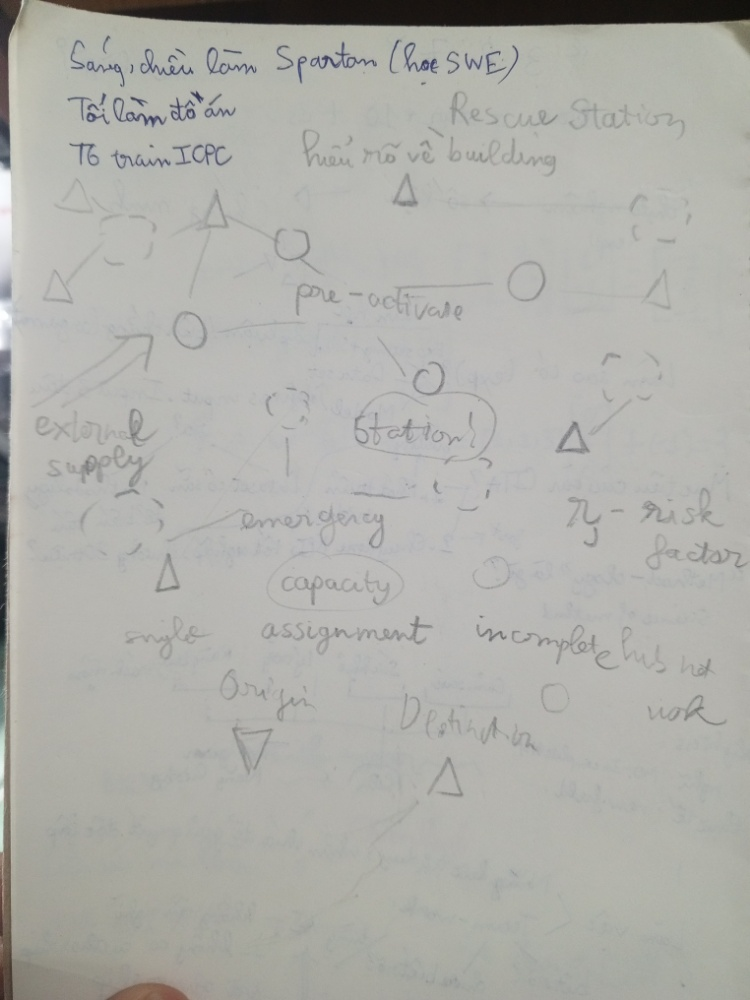
\includegraphics[width=0.5\linewidth]{model-illustration-sketch.png}
    \caption{Illustration of the model}
    \label{fig:placeholder}
\end{figure}
\begin{figure}
    \centering
    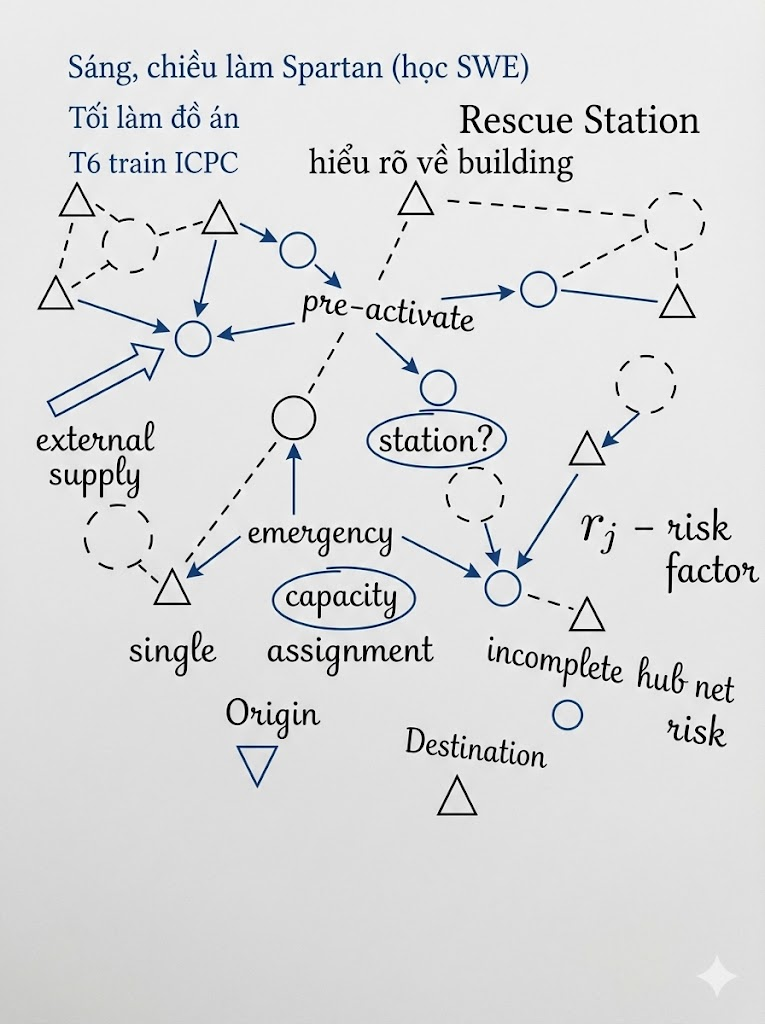
\includegraphics[width=0.5\linewidth]{model-illus-ai.png}
    \caption{AI-generated illustration}
    \label{fig:placeholder}
\end{figure}
}

\section{Problem Description and Mathematical Model}

% TO-DO: Draw a figure for the model and insert it here

To design an efficient disaster relief network (DRND), specifically adjusted for flood disaster response in Central Vietnam, we framed the problem as a multi-objective incomplete hub location network design problem (MO-IHLNDP). This model is the capacitated, single-allocation variant of the HLP. 

The main components of our network are origins, hubs, and demands. In our practical settings, hubs refer to the rescue stations. There are two kinds of hubs, corresponding to two kinds of strategies. The first type is established in advance of the disasters, strategically positioned, and inventoried with amenities. The second type is opened dynamically for disaster response and has high approachability to affected areas. Lastly, during the disaster response, we gradually discover the victim groups, which are referred to as \textbf{demands}. Besides the government's planned forces, some volunteers spontaneously offer to help; these are referred to as \textbf{origins}.

From a practical point of view, DRND involves multiple critical uncertainty factors. 
Firstly, the disruption of transportation infrastructure (e.g., damaged roads and buildings) can easily disable pre-programmed plans, urging the need for a dynamic solution \cite{Yahyaei2019}. 
Secondly, the exact locations of the demands, the total number of victims, and the availability of supply origins are highly uncertain during the rescue process \cite{tofighi2016humanitarian}. 

\mycomment{
From a practical point of view, we can observe many uncertainty factors involved. 
Firstly, traffic infrastructure such as roads or buildings may be damaged and unavailable. 
The disruption of the transportation network may disable many programmed plans, urging the need for a dynamic solution \cite{Yahyaei2019}. 
Secondly, we cannot know in advance the exact positions of demands and may not identify all the victims during the rescue process. 
Furthermore, the exact number of people who need help, as well as the availability of origins, is highly uncertain \cite{tofighi2016humanitarian}.
}

To account for these uncertainties, we employ a two-stage stochastic programming approach utilizing multiple scenarios. 
In each scenario, a specific risk factor is assigned to each area. We also assume that search and rescue (SAR) operations rely heavily on dynamic external supply sources, as pre-positioned hubs may not fully satisfy the uncertain demands under extreme scenarios.

Finally, the model places a strong emphasis on \textit{social equity} by integrating the deprivation cost \cite{holguin2013appropriate}. To obtain a robust approximation of the rescue time from an established hub to its assigned demand points without causing computational intractability, we utilize Daganzo's continuous approximation formula \cite{daganzo2005logistics}, a technique widely adopted in routing problems.

% To account for this, we use a two-stage stochastic programming approach, in which multiple scenarios are considered. In each scenario, a risk factor is assigned to each area. We also assume that the search and rescue (SAR) operations rely on a large proportion of supply coming from external sources, as it is not always the case that the pre-positioned hubs can satisfy all the uncertain demands under extreme scenarios.

% The model also puts \textit{social equity} as one of the main objectives to be optimized by considering the deprivation cost \cite{holguin2013appropriate}. Furthermore, to obtain a robust approximation of the rescue time from an established hub to its assigned demand points, we utilized Daganzo's continuous approximation formula \cite{daganzo2005logistics}, which is widely adopted in the Vehicle Routing Problem.

\subsection{Sets and Indices}
\noindent
\begin{tabular}{l p{0.85\textwidth}}
$\mathcal{H}, \mathcal{I}, \mathcal{J}$ & Set of candidate hubs ($k, h$), demand nodes ($i$), and  origins ($j$) \\
$\mathcal{S}, \mathcal{M}$ & Set of disaster scenarios ($s$) and transportation modes ($m$) \\
$\mathcal{V}$ & Set of all nodes ($u,v$) representing the area in question, $\mathcal{V} = \mathcal{H} \cup \mathcal{I} \cup \mathcal{J}$ \\
\end{tabular}

\subsection{Parameters}

\noindent \textbf{First-Phase Parameters (Strategic Planning)} \\
\begin{tabular}{l p{0.85\textwidth}}
$F_k$ & Fixed cost to establish hub $k$ of the first type (before the disaster) \\
$c_k, \kappa_k$ & Unit holding cost and capacity limit for inventory at hub $k$ \\
$\alpha, \chi, M$ & Discount factor for economies of scale, max acceptable risk threshold, and Big-M constant \\
$C_{uvm}, \tau_{uvm}$ & Unit transportation cost and estimated travel time from node $u$ to $v$ via mode $m$ \\
$C_m, Q_m$ & Unit local routing cost and transportation capacity for vehicle mode $m$ \\
$\gamma$ & Conversion factor (average amount of relief items required per evacuated person) \\
\end{tabular}

% \vspace{0.2cm}
\noindent \textbf{Second-Phase Parameters (Disaster Response, Scenario $s$)} \\
\begin{tabular}{l p{0.85\textwidth}}
$\pi_s$ & Probability of scenario $s$ \\
$F_{ks}^{a}$ & Fixed cost to establish hub $k$ of the second type (reactive) in scenario $s$ \\
$\tau_{ks}$ & Processing time for each rescue round trip at hub $k$ in scenario $s$ \\
$a_{uvms}$ & Accessibility of arc $(u,v)$ via mode $m$ in scenario $s$ (1 if traversable, 0 otherwise) \\
$r_{us}, \lambda_{is}$ & Risk index of node $u$, and deprivation sensitivity coefficient for demand $i$ in scenario $s$ \\
$D_{is}, O_{js}$ & Demand (number of people to evacuate) at $i$, and relief items provided at origin $j$ in scenario $s$ \\
$\Theta_{kis}$ & Pre-computed CA routing cost to execute the evacuation from grid $i$ to hub $k$ in scenario $s$ \\
$\Phi, \eta, A_i$ & Daganzo's circuity factor, average group size per distress location, and area of grid cell $i$ \\
\end{tabular}

\subsection{Decision Variables}
\noindent
\begin{tabular}{l p{0.85\textwidth}}
$x_{k} \in \{0,1\}$ & 1 if hub $k$ is established as the first type (planned), 0 otherwise \\
$y_{ks} \in \{0,1\}$ & 1 if hub $k$ is established as the second type (reactive) in scenario $s$, 0 otherwise \\
$z_{iks} \in \{0,1\}$ & 1 if demand $i$ is assigned to be evacuated to hub $k$ in scenario $s$, 0 otherwise \\
$z_{jks} \in \{0,1\}$ & 1 if origin $j$ supplies hub $k$ in scenario $s$, 0 otherwise \\
$q_{k} \ge 0$ & Amount of relief items inventoried at hub $k$ \\
$f_{khms} \ge 0$ & Lateral trans-shipment flow volume from hub $k$ to hub $h$ via mode $m$ in scenario $s$ \\
\end{tabular}

\subsection{Objectives}
\textbf{Objective 1: Minimize Total Expected Logistics Cost ($Z_1$)}

\begin{equation} \label{eq:obj1}
\begin{aligned}
    \text{Min } Z_1 = & \underbrace{\sum_{k \in \mathcal{H}} F_k x_k + \sum_{k \in \mathcal{H}} c_k q_k}_{\text{Pre-disaster strategic costs}} \\
    & + \sum_{s \in \mathcal{S}} \pi_s \Bigg[ \underbrace{\sum_{k \in \mathcal{H}} F_{ks}^a y_{ks}}_{\text{Reactive setup}} 
    + \underbrace{\sum_{j \in \mathcal{J}} \sum_{k \in \mathcal{H}} \left( \min_{m \in \mathcal{M} \mid a_{jkms}=1} C_{jkm} \right) O_{js} z_{jks}}_{\text{Origin to Hub supply flow}} \\
    % + \underbrace{\sum_{j \in \mathcal{J}} \sum_{k \in \mathcal{H}} \sum_{m \in \mathcal{M}} C_{jkm} O_{js} z_{jks}}_{\text{Origin to Hub supply flow}} \\
    & + \underbrace{\sum_{k \in \mathcal{H}} \sum_{h \in \mathcal{H}} \sum_{m \in \mathcal{M}} \alpha C_{khm} f_{khms}}_{\text{Inter-hub lateral trans-shipment}} 
    + \underbrace{\sum_{k \in \mathcal{H}} \sum_{i \in \mathcal{I}} \Theta_{kis} z_{iks}}_{\text{Grid-based Last-Mile CA}} 
    \Bigg]
\end{aligned}
\end{equation}

Objective $Z_1$ minimizes the total expected logistics cost, balancing pre-disaster investments against reactive setups and transportation costs. To have an accurate estimation of last-mile evacuation cost while keeping the model simple, we adopted Daganzo's Continuous Approximation \cite{daganzo2005logistics}. The region of interest is partitioned via spatial discretization, and the demands are aggregated on a grid basis. The routing cost $\Theta_{kis}$ is pre-computed as a parameter:
\begin{equation*} \label{eq:daganzo_theta}
    \Theta_{kis} = \min_{m \in \mathcal{M}} \left( 2 \cdot C_{kim} \cdot \lceil D_{is}/Q_m \rceil + C_{m} \cdot \Phi \sqrt{\lceil D_{is}/\eta \rceil \cdot A_i} \right)
\end{equation*}

\textbf{ Objective 2: Minimize Expected Maximum Deprivation Cost ($Z_2$)}

% Formula: max (s over S) (sum i over I) IS CHANGED TO avg (s over S) (max i over I)
% \begin{equation} \label{eq:obj2}
% \text{Min } Z_2 = \max_{s \in \mathcal{S}} \left( \sum_{i \in \mathcal{I}} D_{is} \cdot \left( e^{\lambda_{is} \cdot \Omega_{is}} - 1 \right) \right)
% \end{equation}

\begin{equation} \label{eq:obj2}
    \text{Min } Z_2 = \sum_{s \in \mathcal{S}} \pi_s \left( \max_{i \in \mathcal{I}} \left[ D_{is} \cdot \left( e^{\lambda_{is} \cdot \Omega_{is}} - 1 \right) \right] \right)
\end{equation}

The second objective ensures social equity by minimizing the expected maximum deprivation cost across all scenarios. Based on Holguín-Veras et al. \cite{holguin2013appropriate}, $Z_2$ adopts an exponential function to penalize long waiting times ($\Omega_{is}$) for victims. Furthermore, it forces the model to distribute resources evenly, ensuring overall low delay time for everyone.

\begin{equation*} \label{eq:waiting_time}
\Omega_{is} = \sum_{k \in \mathcal{H}} z_{iks} \left( \tau_{ks} + 2 \cdot \min_{m \in \mathcal{M}} \tau_{kim} \right)
\end{equation*}

The sensitivity coefficient $\lambda_{is}$ is proportional to the risk index $r_{is}$ ($\lambda_{is} = \lambda_0(1 + r_{is})$), effectively prioritizing vulnerable populations. Although $Z_2$ introduces non-linearity, our meta-heuristic solution approach can directly evaluate it as a fitness function. For linearization into a Mixed-Integer Linear Programming (MILP) form, one can exploit the single-allocation property ($\sum_{k \in \mathcal{H}} z_{iks} = 1$).

\subsection{Constraints}

The complete MO-IHLNDP model is formally stated as follows:

\allowdisplaybreaks
\begin{align}
    \text{Minimize } \quad & Z_1, Z_2 \nonumber \\
    \text{subject to} \quad & \text{Constraints } \eqref{eq:hub_type} - \eqref{eq:nonneg_vars} \nonumber \\
    x_k + y_{ks} & \le 1 \quad \forall k \in \mathcal{H}, s \in \mathcal{S} \label{eq:hub_type} \\
    q_k & \le \kappa_k \cdot x_k \quad \forall k \in \mathcal{H} \label{eq:hub_inv_cap} \\
    r_{ks} \cdot (x_k + y_{ks}) & \le \chi \quad \forall k \in \mathcal{H}, s \in \mathcal{S} \label{eq:hub_safety} \\
    \sum_{k \in \mathcal{H}} z_{iks} & = 1 \quad \forall i \in \mathcal{I}, s \in \mathcal{S} \label{eq:single_alloc_demand} \\
    \sum_{k \in \mathcal{H}} z_{jks} & = 1 \quad \forall j \in \mathcal{J}, s \in \mathcal{S} \label{eq:single_alloc_origin} \\
    z_{iks} & \le x_k + y_{ks} \quad \forall i \in \mathcal{I}, k \in \mathcal{H}, s \in \mathcal{S} \label{eq:valid_assign_demand} \\
    z_{jks} & \le x_k + y_{ks} \quad \forall j \in \mathcal{J}, k \in \mathcal{H}, s \in \mathcal{S} \label{eq:valid_assign_origin} \\
    z_{iks} & \le \sum_{m \in \mathcal{M}} a_{ikms} \quad \forall i \in \mathcal{I}, k \in \mathcal{H}, s \in \mathcal{S} \label{eq:path_demand} \\
    z_{jks} & \le \sum_{m \in \mathcal{M}} a_{jkms} \quad \forall j \in \mathcal{J}, k \in \mathcal{H}, s \in \mathcal{S} \label{eq:path_origin} \\
    f_{khms} & \le M \cdot a_{khms} \quad \forall k, h \in \mathcal{H}, m \in \mathcal{M}, s \in \mathcal{S} \label{eq:trans_path} \\
    % \sum_{i \in \mathcal{I}} \gamma D_{is} z_{iks} + \sum_{h \in \mathcal{H}} \sum_{m \in \mathcal{M}} f_{khms} & \le q_k + \sum_{j \in \mathcal{J}} O_{js} z_{jks} + \sum_{h \in \mathcal{H}} \sum_{m \in \mathcal{M}} f_{hkms} \quad \forall k \in \mathcal{H}, s \in \mathcal{S} \label{eq:flow_balance} \\
    \begin{split}
        \sum_{i \in \mathcal{I}} \gamma D_{is} z_{iks} + \sum_{h \in \mathcal{H}} \sum_{m \in \mathcal{M}} f_{khms} & \le q_k + \sum_{j \in \mathcal{J}} O_{js} z_{jks} \\
        & \quad + \sum_{h \in \mathcal{H}} \sum_{m \in \mathcal{M}} f_{hkms} \quad \forall k \in \mathcal{H}, s \in \mathcal{S} 
    \end{split} \label{eq:flow_balance} \\
    q_k + \sum_{j \in \mathcal{J}} O_{js} z_{jks} + \sum_{h \in \mathcal{H}} \sum_{m \in \mathcal{M}} f_{hkms} & \le \kappa_k \cdot (x_k + y_{ks}) \quad \forall k \in \mathcal{H}, s \in \mathcal{S} \label{eq:throughput_cap} \\
    x_k, y_{ks}, z_{iks}, z_{jks} & \in \{0, 1\} \quad \forall i, j, k, s \label{eq:binary_vars} \\
    q_k, f_{khms} & \ge 0 \quad \forall k, h, m, s \label{eq:nonneg_vars}
\end{align}

Constraints \eqref{eq:hub_type} define
the hub establishment. For planned hubs, inventory is bounded by physical capacity \eqref{eq:hub_inv_cap}, while the reactive hubs are required to be placed within safe zones \eqref{eq:hub_safety}.
Constraints \eqref{eq:single_alloc_demand}-\eqref{eq:path_origin} rigorously enforce the single-allocation property to active hubs via available links. 
Constraint \eqref{eq:trans_path} restricts flow to be trans-shipped on intact paths. 
Constraints \eqref{eq:flow_balance} and \eqref{eq:throughput_cap} maintain flow conservation and capacity limits. Specifically, \eqref{eq:flow_balance} ensures that total supply, comprising inventory ($q_k$), external origins ($O_{js}$), and incoming flows -- satisfies both victim demand (converted by $\gamma$) and outgoing trans-shipments.
Variable domains are defined in \eqref{eq:binary_vars}-\eqref{eq:nonneg_vars}.

\section{Proposed Algorithm: PB-NSGA-II}

The MO-IHLNDP is NP-hard due to its combinatorial structure and non-linear $Z_2$. Exact solvers are intractable beyond small instances. We therefore propose the \textbf{Priority-Based NSGA-II (PB-NSGA-II)}. It integrates a custom decoding heuristic into the NSGA-II framework \cite{deb2002fast}. 

The key design principle is \emph{implicit encoding}. Only first-stage strategic variables are encoded in the chromosome. All second-stage variables are reconstructed deterministically by the decoder for each scenario $s \in \mathcal{S}$. This drastically reduces the search space from $O(|\mathcal{S}| \times |\mathcal{V}|)$ to $O(|\mathcal{H}|)$.

\subsection{Chromosome Encoding}


Each chromosome $\mathbf{C} = (\mathbf{X}, \mathbf{R}, \mathbf{W})$ encodes three segments:
\begin{itemize}
    \item $\mathbf{X} \in \{0,1\}^{|\mathcal{H}|}$: binary hub activation vector. $X_k=1$ if and only if hub $k$ is planned before the disaster.
    \item $\mathbf{R} \in [0,1]^{|\mathcal{H}|}$: inventory ratio vector. The absolute pre-positioned inventory is decoded as:
    \begin{equation*}
        q_k = R_k \cdot \frac{\hat{D}}{n_{\text{open}}}, \quad n_{\text{open}} = \textstyle\sum_{k} X_k,
    \end{equation*}
    where $\hat{D} = \gamma \cdot \max_{s}\sum_{i} D_{is}$ is the worst-case total demand in kg. This encoding ensures complete coverage. When $R_k = 1$ for all open hubs, the combined inventory exactly covers the worst-case demand. Capacity $\kappa_k$ acts as a soft upper bound.
    \item $\mathbf{W} = (w_1, w_2, w_3) \in [0,1]^3$: heuristic weight vector. It governs the priority scoring during decoding.
\end{itemize}

\subsection{Priority-Based Decoding Heuristic}


The decoder is invoked for each scenario $s$. It proceeds through four steps:

\textbf{Step 1 -- Hub Activation.} Planned hubs ($X_k=1$) with risk $r_{ks} \le \chi$ are activated. If no planned hub is safe, the hub with the lowest risk is activated reactively. Additional reactive hubs ($y_{ks}=1$) may be activated later for unserviceable demand nodes.

\textbf{Step 2 -- Priority-Based Demand Assignment.} Each demand node $i$ is assigned a priority score:
\begin{equation*}
    \text{Score}_i = w_1 \cdot (\lambda_{is} \cdot D_{is}) - w_2 \cdot \min_{k \in \text{active}} \tau_{ikm^*},
\end{equation*}
where $m^* = \arg\min_m \tau_{ikm}$ subject to $a_{ikms}=1$. Demands are sorted descendingly. They are assigned greedily to the highest-scoring active hub reachable via at least one mode. If no active hub can reach demand $i$, a reactive hub is opened from among safe candidates. Failing that, a constraint violation (CV) penalty of $\gamma D_{is}$ is incurred.

\textbf{Step 3 -- Origin Assignment and Flow Balancing.} Each origin $j$ is routed to the nearest active hub. A greedy trans-shipment loop then iteratively routes relief from surplus hubs to deficit hubs. It uses the cheapest available mode and incorporates the economies-of-scale discount $\alpha$. Remaining deficits contribute proportionally to the CV score.

\textbf{Step 4 -- Objective Evaluation.} $Z_1$ and $Z_2$ are accumulated as weighted expectations over scenarios using Equations (\ref{eq:obj1}) and (\ref{eq:obj2}). The deprivation waiting time is $\Omega_{is} = \tau_{ks} + 2\tau_{ikm^*}$. It is capped to prevent numerical overflow.

\subsection{Genetic Operators and Selection}

The mixed-type chromosome requires mode-specific operators. \emph{Selection} uses a binary tournament on rank and crowding distance. \emph{Crossover} ($p_c = 0.9$) utilizes Uniform Crossover for $\mathbf{X}$ and Simulated Binary Crossover (SBX, $\eta_c = 20$) for $\mathbf{R}$ and $\mathbf{W}$. \emph{Mutation} ($p_m \propto 1/|\mathbf{C}|$) applies Bit-flip for $\mathbf{X}$ and Polynomial mutation ($\eta_m = 20$) for $\mathbf{R}$ and $\mathbf{W}$. 

Constraint handling follows the constrained-dominance principle. Infeasible solutions (CV $> 0$) are always dominated by feasible ones. Among infeasible solutions, a lower CV dominates. The Pareto archive uses fast non-dominated sorting with crowding distance tie-breaking.

\section{Computational Experiments}

\subsection{Experimental Setup}

\textbf{Implementation.} PB-NSGA-II is implemented in C++17. Data generation and result analysis are performed in Python 3. All experiments run on a standard workstation (Intel Core i7, 16 GB RAM).

\textbf{Algorithm parameters.} Population $N = 100$; generations $G = 200$; $p_c = 0.9$; $\eta_c = \eta_m = 20$; $p_m = 1/|\mathbf{C}|$. The safety threshold is $\chi = 0.7$; discount $\alpha = 0.6$; $\gamma = 3.0$ kg/person; $\lambda_0 = 0.8$.

\textbf{Performance metric.} We use the \textbf{Hypervolume (HV)} indicator. The reference point is set to $1.1 \times \max(Z_1, Z_2)$ of the combined Pareto front. A larger HV indicates better coverage and spread of the Pareto front.

\subsection{Dataset Description}


\textbf{Benchmark datasets.} We adapt two widely-used hub location benchmarks: the \textbf{AP} set \cite{ap_dataset} (Euclidean instances of sizes 10--100 nodes) and \textbf{TR81} \cite{tr81_dataset} (Turkish inter-city matrix, 81 nodes). Each benchmark is transformed into a DRND instance. We assign hub/origin/demand roles and generate three flood scenarios (mild, severe, extreme) with probabilities $(\pi_1, \pi_2, \pi_3) = (0.60, 0.30, 0.10)$. Supply and demand are calibrated to $1.5$--$2.5\times$ total demand coverage. Road distances are normalized to a 500 km scale. Three transport modes operate concurrently (Table~\ref{tab:modes}).

\begin{table}[ht]
\centering
\caption{Transport mode parameters.}
\label{tab:modes}
\begin{tabular}{llrrrr}
\toprule
Mode & Vehicle & Speed (km/h) & Cost (\$/km) & Capacity (pers.) & Disruption \\
\midrule
0 & Truck       & 35  & 2.0  & 60 & Road-dependent \\
1 & Motorboat   & 25  & 5.0  & 25 & Low (flood-resilient) \\
2 & Helicopter  & 150 & 40.0 & 10 & None (always available) \\
\bottomrule
\end{tabular}
\end{table}

\textbf{Central Vietnam case study.} We generate two synthetic instances modelling the flood-prone \textbf{Vu Gia -- Thu Bon} river basin (Da Nang -- Quang Nam region):
\begin{itemize}
    \item \textbf{CV-Small}: $|\mathcal{I}|=20$, $|\mathcal{H}|=5$, $|\mathcal{J}|=2$, $|\mathcal{S}|=3$ -- small-scale planning instance.
    \item \textbf{CV-Large}: $|\mathcal{I}|=100$, $|\mathcal{H}|=20$, $|\mathcal{J}|=12$, $|\mathcal{S}|=3$ -- high-resolution regional instance.
\end{itemize}
Node coordinates are drawn from real geographic locations. Road travel times are estimated via the OSRM API with a terrain-adjusted cost factor for inland areas. Scenario epicenters are sampled from flood-prone sub-regions. Risk indices decay with distance from the epicenter. Hub capacities are calibrated post-scenario generation to ensure structural feasibility ($\kappa_k \ge 3\hat{D}/|\mathcal{H}|$).

\subsection{Results}

Table~\ref{tab:hv_benchmark} reports the final-generation hypervolume for each instance. For benchmark instances, we run one seed ($G=200$, $N=100$). For CV-Small, we run three independent seeds to assess robustness.

\begin{table}[ht]
\centering
\caption{Hypervolume (HV) results across all instances. CV-Small reports mean over 3 seeds.}
\label{tab:hv_benchmark}
\begin{tabular}{llrr}
\toprule
Category & Instance & \#Pareto pts & HV \\
\midrule
\multirow{6}{*}{AP Benchmark}
    & AP10  & 100 & $1.17 \times 10^{14}$ \\
    & AP20  & 100 & $6.77 \times 10^{14}$ \\
    & AP25  & 100 & $2.20 \times 10^{13}$ \\
    & AP40  & 100 & $9.87 \times 10^{13}$ \\
    & AP50  & 100 & $4.94 \times 10^{13}$ \\
    & AP100 &  25 & $2.65 \times 10^{14}$ \\
\midrule
TR Benchmark & TR81 & 2 & $3.20 \times 10^{13}$ \\
\midrule
\multirow{2}{*}{Case Study}
    & CV-Small ($n=3$) & 152 (combined) & $1.01 \times 10^{12}$ \\
    & CV-Large         & 100            & $3.23 \times 10^{13}$ \\
\bottomrule
\end{tabular}
\end{table}



\textbf{Benchmark observations.} The algorithm consistently produces well-spread Pareto fronts across all AP instances. AP20 yields the largest HV. This reflects the favourable trade-off structure of mid-size instances. AP100 produces fewer non-dominated points (25). This is expected as the search landscape becomes harder and population diversity is consumed. TR81 converges to only 2 non-dominated solutions. It indicates a strong dominance structure where a single hub configuration dominates most others in a dense graph.

\textbf{Case study observations.} For CV-Small, a combined Pareto front of 152 points demonstrates excellent solution diversity and reproducibility. CV-Large achieves 100 non-dominated solutions with an HV comparable to TR81. This illustrates that PB-NSGA-II scales effectively to large real-world instances. The smaller HV relative to AP benchmarks is attributable to the narrow feasible region. The flood disruption model severely restricts options (e.g., only 3 out of 5 hubs remain safe in extreme scenarios).

\subsection{Managerial Insights}

Analyzing the Pareto front of CV-Small reveals a clear convex trade-off. Reducing $Z_2$ (deprivation) by 30\% requires increasing $Z_1$ (logistics cost) by approximately $3\times$. This reflects the exponential structure of the deprivation function. Reducing waiting times for high-risk isolated areas is disproportionately costly.



Network topology analysis further highlights structural shifts. Under the \textit{mild} scenario, the optimal strategy uses road transport from all 5 candidate hubs with moderate inventory pre-positioning. Under the \textit{extreme} scenario, 2 hubs become unsafe ($r_{ks} > \chi$). The network dynamically switches to water and air transport. The remaining active hubs receive larger inventory pre-commitments. This is compensated by increased lateral trans-shipment. This shift confirms the value of the two-stage stochastic formulation. A deterministic single-scenario model would systematically under-invest in network resilience.

\section{Conclusion and Future Work}

We proposed PB-NSGA-II for the Multi-Objective Incomplete Hub Location Network Design Problem (MO-IHLNDP). The model incorporates multi-modal transport, stochastic flood scenarios, deprivation cost, and Daganzo's continuous approximation. Our priority-based decoding scheme efficiently handles second-stage variables and maintains feasibility in disrupted networks. Experiments on AP and TR81 benchmarks validate the algorithm's effectiveness. The Central Vietnam case study demonstrates its practical applicability.

\textbf{Limitations.} The current model relies on a fixed set of pre-defined scenarios. The decoding heuristic is greedy and may miss globally optimal demand assignments. 

\textbf{Future work} will explore exact branch-and-cut approaches for small instances to establish lower bounds. We also aim to incorporate real-time sensor data via online re-optimization and extend the framework to multi-period relief operations.

\mycomment{

\section{Proposed Algorithm (W.I.P., done up to Encoding)}

The formulated MO-IHLNDP is highly complex. Exact solvers struggle with large instances and non-linear properties. Therefore, we propose the Priority-Based Non-dominated Sorting Genetic Algorithm (PB-NSGA-II). 

\\subsection{Overview of the meta-heuristic framework}
NSGA-II \cite{deb2002fast} is a multi-objective evolutionary algorithm well-known for its efficiency across a wide range of industrial problems. It relies on non-dominated sorting and crowding distance to maintain a diverse Pareto front. We utilize this core framework. However, encoding all variables of a two-stage stochastic problem expands the search space exponentially. To resolve this, only the first-stage strategic decisions and heuristic strategy weights are encoded in PB-NSGA-II. The scenario-dependent second-stage variables are then derived via a custom decoding heuristic, using the encoded information.

\subsection{Encoding scheme}

In GA, a chromosome encodes the decision variables and the implied solution in its representation. The chromosome in PB-NSGA-II is designed as a collection of arrays corresponding to three pieces of information:
\begin{itemize}
    \item Activated Hubs of the first type ($X$): A binary array of length $|\mathcal{H}|$, where $X_k = 1$ indicates hub $k$ is established before the disaster.
    \item Inventory level ($Q$): An array of continuous variables of length $|\mathcal{H}|$. $Q_k$ represents the proportions of the forecasted total demand covered by hub $k$.
    \item Heuristic weights ($W$): Consists of the weights ($w_1, w_2, w_3, w_4 \in [0,1]$). They guide second-stage decisions by respectively adjust the importance of sensitivity coefficient, demand deprivation, distance to nearest hub, and supply scarcity.
\end{itemize}

\subsection{Decoding heuristic}

This mechanism is the core of our proposed algorithm. It translates the genotype into operational phenotypes across all scenarios $s \in \mathcal{S}$. It also calculates the objective values $Z_1$ and $Z_2$. The complete priority-based decoding procedure is detailed in Algorithm \ref{alg:decoding}.



\begin{algorithm}[htbp]
\caption{Two-Stage Priority-Based Decoding Heuristic}
\label{alg:decoding}
\begin{algorithmic}[1]
\REQUIRE Chromosome $C = (X, Q, W)$, Scenarios $\mathcal{S}$, Parameters
\ENSURE Total Logistics Cost $Z_1$, Expected Max Deprivation Cost $Z_2$, Constraint Violation $CV$
\STATE Initialize $Z_1 \leftarrow 0$, $Z_2 \leftarrow 0$, $CV \leftarrow 0$
\STATE Forecast total regional demand $D_{total}$
\STATE \textbf{// Phase 1: Strategic Instantiation}
\FOR{each candidate hub $k \in \mathcal{H}$}
    \STATE Set $x_k \leftarrow X_k$
    \STATE \textbf{if} $x_k = 1$ \textbf{then} $q_k \leftarrow Q_k \cdot D_{total}$ \textbf{else} $q_k \leftarrow 0$
\ENDFOR
\STATE Normalize $q_k$ to satisfy total inventory constraints.
\STATE Add first-stage fixed and holding costs to $Z_1$.
\STATE \textbf{// Phase 2: Scenario Evaluation}
\FOR{each scenario $s \in \mathcal{S}$}
    \STATE Initialize Active Hubs $\mathcal{H}_{act} \leftarrow \{k \mid x_k = 1 \text{ and } r_{ks} \le \chi \}$
    \STATE \textbf{// Reactive Setup}
    \IF{total capacity of $\mathcal{H}_{act} < \sum_i D_{is}$}
        \STATE Sort inactive hubs by $w_4 \cdot r_{ks}$ (ascending).
        \STATE Open reactive hubs ($y_{ks} \leftarrow 1$) until capacity is met. Add to $\mathcal{H}_{act}$.
    \ENDIF
    \STATE Add reactive setup costs to $Z_1$.
    \STATE \textbf{// Priority Allocation}
    \FOR{each demand $i \in \mathcal{I}$}
        \STATE $Dist \leftarrow \min_{k \in \mathcal{H}_{act}} (\text{distance to } k)$
        \STATE $Score_i \leftarrow w_1(D_{is}\lambda_{is}) + w_2(r_{is}) - w_3(Dist)$
    \ENDFOR
    \STATE Sort $\mathcal{I}$ descendingly by $Score_i$.
    \STATE Greedily assign ($z_{iks} \leftarrow 1$) each sorted $i$ to the nearest valid hub in $\mathcal{H}_{act}$.
    \STATE If unassigned, increment $CV$. Add Daganzo CA routing costs to $Z_1$.
    \STATE Compute deprivation cost $Dep_s$ for all assigned demands.
    \STATE \textbf{// Flow Balancing}
    \STATE Assign origins ($z_{jks} \leftarrow 1$) to nearest hubs in $\mathcal{H}_{act}$.
    \STATE Compute net inventory for all $k \in \mathcal{H}_{act}$.
    \STATE Greedily route trans-shipment flows ($f_{khms}$) from surplus to deficit hubs.
    \STATE If deficits remain, increment $CV$. Add trans-shipment costs to $Z_1$.
    \STATE $Z_2 \leftarrow Z_2 + \pi_s \cdot \max_i (Dep_s)$
\ENDFOR
\RETURN $Z_1, Z_2, CV$
\end{algorithmic}
\end{algorithm}

\noindent \textbf{Decoding Mechanism Explanation:} \\
Algorithm \ref{alg:decoding} maps the encoded variables into feasible network structures. Phase 1 handles the static pre-disaster decisions. It determines planned hubs and allocates absolute inventory. Phase 2 simulates the dynamic disaster response. It iterates through all scenarios to deploy reactive operations. A scoring function drives the demand allocation. It heavily prioritizes highly vulnerable clusters using the encoded weights. A greedy heuristic then resolves the lateral trans-shipments. Disasters often cause severe link failures. If demands remain isolated or hubs face shortages, the algorithm increments a Constraint Violation (CV) counter. The NSGA-II framework uses this CV score. It strictly penalizes infeasible solutions via the constrained-domination principle.



\subsection{Two-Stage Priority-Based Decoding}
This mechanism is the core of our proposed algorithm. It translates the genotype into operational phenotypes across all scenarios $s \in \mathcal{S}$. It also calculates the objective values $Z_1$ and $Z_2$. For each chromosome, the decoding process follows these sequential steps:

\begin{enumerate}
    \item \textbf{Strategic Instantiation:} We read array $X$ to open planned hubs. We calculate the absolute inventory $q_k$ by multiplying array $Q$ with a forecasted total regional demand. If $x_k = 0$, we force $q_k = 0$ and normalize the remaining ratios.
    \item \textbf{Reactive Setup:} For each scenario $s$, we evaluate the capacity of active planned hubs. If the capacity is insufficient, we open reactive hubs ($y_{ks} = 1$). Candidate nodes are prioritized by their risk index $r_{ks}$ using weight $w_4$. Nodes exceeding the safety threshold $\chi$ are strictly ignored.
    \item \textbf{Priority Allocation:} We assign a priority score to each demand node $i$. The score formula is $Score_i = w_1(D_{is}\lambda_{is}) + w_2(r_{is}) - w_3(Dist)$, where $Dist$ is the distance to the nearest active hub. We sort demands descendingly based on this score. Demands are then greedily assigned ($z_{iks}$) to the nearest hub with available capacity and valid paths ($a_{ikms}=1$).
    \item \textbf{Flow Balancing:} Origins are assigned ($z_{jks}$) to their nearest active hubs. We compute the net inventory at each hub. A greedy heuristic then routes trans-shipment flows ($f_{khms}$) from surplus hubs to deficit hubs via the cheapest available links.
    \item \textbf{Penalty Handling:} Disasters often cause severe disruptions. If demands remain unassigned or hubs face inventory deficits, we calculate a Constraint Violation (CV) score. We use the constrained-domination principle of NSGA-II to heavily penalize these infeasible solutions.
\end{enumerate}



\section{Computational Experiments}
To evaluate the proposed MO-IHLNDP model and algorithms, we conduct a series of computational experiments. The algorithms are strictly implemented in C++. Data preprocessing and visualizations are handled using Python. All experiments run on a standard machine with an Intel Core i7 CPU and 16GB RAM.

\subsection{Data Generation and Scenarios}
We generate a semi-real dataset reflecting the flood-prone Vu Gia -- Thu Bon river basin in Central Vietnam. Candidate hubs, demand clusters, and supply origins are distributed within this geographical bounding box. We utilize the Open Source Routing Machine (OSRM) API. This extracts real-world road distances and travel times. 

To capture the stochastic nature of disasters, we define three disruption scenarios. Table \ref{tab:scenarios} summarizes the scenario parameters.
% [TODO: INSERT TABLE 1 - Scenario Configurations HERE]

Scenario S1 represents a mild flood. It maintains high infrastructure availability (95\% active links) and low risk indices. Scenario S2 depicts a severe flood causing moderate road disruptions (30\% links disrupted). Scenario S3 represents an extreme typhoon event. In S3, the network faces severe link failures (60\% disrupted) and peak risk indices.

\subsection{Algorithmic Settings}
We evaluate two versions of the solver: the baseline PB-NSGA-II and the proposed NSMA (integrating Local Search). The population size is set to 100. The maximum number of generations is 200. The crossover rate is 0.9. The mutation rate is 0.1. We execute each algorithm for 10 independent runs. A fixed random seed is used to ensure full reproducibility.
% [TODO: INSERT TABLE 2 - Algorithm Parameters HERE]

\subsection{Trade-off Analysis and Results}
Figure \ref{fig:pareto} illustrates the Pareto fronts obtained by the algorithms. 
% [TODO: INSERT FIGURE 1 - Pareto Front Scatter Plot HERE]

[PLACEHOLDER FOR RESULTS: The Pareto front demonstrates a clear conflict between the two objectives. Minimizing the expected deprivation cost ($Z_2$) requires a massive exponential increase in logistics costs ($Z_1$). Our proposed NSMA effectively dominates the baseline NSGA-II. The local search mechanism successfully refines the boundaries of the non-dominated solutions. We identify a knee-point solution. This point provides the most balanced trade-off for decision-makers.]

% [TODO: INSERT TABLE 3 (Optional) - Hypervolume & CPU Time HERE]

\subsection{Managerial Insights on Network Resilience}
We extract the knee-point solution to analyze the network topology. Figure \ref{fig:topology} displays the routing and hub activation differences across scenarios.
% [TODO: INSERT FIGURE 2 - Network Topology Maps HERE]

[PLACEHOLDER FOR INSIGHTS: The network dynamically adapts to the disruption severity. In scenario S1, the system relies heavily on road networks and scattered reactive hubs. In scenario S3, severe road disruptions occur. The system automatically switches to water-based transportation. Relief flows are consolidated into highly secure, pre-positioned type-1 hubs. This structural shift highlights the robustness of our two-stage stochastic approach. It proves that static single-scenario planning is inadequate for extreme disasters.]

}

% \begin{credits}

% \subsubsection{\ackname} This work is under the support of Vietnam - Korea University of Information and Communication.

% % \subsubsection{\discintname}
% % The authors have no competing interests to declare that are
% % relevant to the content of this article. 

% \end{credits}

\bibliographystyle{splncs04}
\bibliography{cite-class.bib}


\end{document}
